\documentclass[12pt]{article}
\usepackage[a4paper, total={6in, 8in}]{geometry}
\usepackage[utf8]{inputenc}
\usepackage{booktabs}
\usepackage{rotating}
\usepackage{multirow}
\usepackage[graphicx]{realboxes}
\usepackage{stackengine}
\usepackage{epigraph}
\usepackage{float}
\usepackage{dcolumn}
% \usepackage{longtable}
\usepackage{supertabular}
% \usepackage[nomarkers]{endfloat}
\usepackage{acronym}
\usepackage{listings}
\usepackage{hyperref}
\hypersetup{colorlinks=true,%
citecolor=black,%
filecolor=black,%
linkcolor=black,%
urlcolor=black
}
\usepackage[portuguese]{babel}
\usepackage[autostyle,portuguese=brazilian]{csquotes}
\usepackage{setspace} % for \onehalfspacing and \singlespacing macros
\onehalfspacing
\usepackage{etoolbox}
\usepackage{amsmath}
\AtBeginEnvironment{quote}{\singlespacing\small}
% \usepackage[usestackEOL]{stackengine}
\usepackage[justification=centering]{caption}
\usepackage[notes,backend=biber]{biblatex-chicago}
\usepackage{subfig} %incluir Figura side by side
%codigo  para spacing 1.5
%\usepackage{setspace}
%\doublespacing
%codigo para monospace justificado tt
\renewcommand{\familydefault}{\rmdefault}
%codigo estilo dos numeros
\usepackage[sc,osf]{mathpazo}
\usepackage{ragged2e}
\justifying

\usepackage{listings}
\usepackage{xcolor}

\definecolor{codegreen}{rgb}{0,0.6,0}
\definecolor{codegray}{rgb}{0.5,0.5,0.5}
\definecolor{codepurple}{rgb}{0.58,0,0.82}
\definecolor{backcolour}{rgb}{0.95,0.95,0.92}

\lstdefinestyle{mystyle}{
    backgroundcolor=\color{backcolour},   
    commentstyle=\color{codegreen},
    keywordstyle=\color{magenta},
    numberstyle=\tiny\color{codegray},
    stringstyle=\color{codepurple},
    basicstyle=\ttfamily\footnotesize,
    breakatwhitespace=false,         
    breaklines=true,                 
    captionpos=b,                    
    keepspaces=true,                 
    numbers=left,                    
    numbersep=5pt,                  
    showspaces=false,                
    showstringspaces=false,
    showtabs=false,                  
    tabsize=2
}

\lstset{style=mystyle}

\bibliography{references.bib}

\usepackage{enumitem}
\newlist{floatnotes}{description}{1}
\setlist[floatnotes]{font=\normalfont\itshape,wide, nosep, leftmargin=.1\linewidth, itemindent=\labelsep, rightmargin=\leftmargin, before=\vspace{.5em}\footnotesize}

\usepackage{pdflscape}
\usepackage{afterpage}
\usepackage{capt-of}% or use the larger `caption` package
\usepackage{enumitem}

\makeatletter
%Add packages here
\usepackage{hyperref}

\begin{document} 

\newgeometry{margin = .65in, top=1.05in}
\linespread{1.1}

\title{%
  A mulher negra no mercado de trabalho brasileiro: desigualdades salariais, representatividade e educação entre 2010 e 2022\\
  \vspace{1cm}
  \Large \texttt{\MakeUppercase{DRAFT}}}

\author{Pacto de Promoção da Equidade Racial \thanks{Responsáveis técnicos: Crislane Alves e Lucas Cavalcanti Rodrigues}}


\maketitle

\section{Introdução}

\par Este texto de discussão tem como objetivo analisar as condições de participação da mulher negra no mercado de trabalho brasileiro no período entre os anos de 2010 e 2022. Tendo em vista a amplitude do tema sob discussão, maior atenção será dada a dimensões previamente selecionadas, nomeadamente, desigualdades salariais, representatividade e educação.

\par Em termos gerais, o presente estudo corrobora achados da literatura sobre o tema e indica novos achados que podem servir de base para investigações mais aprofundadas. No âmbito do diálogo com a literatura existente, o texto retoma e atualiza fatos estilizados ao mostrar que a mulher negra encontra-se em posição mais desfavorável, tanto em termos salariais quanto de representatividade, em relação aos demais sub-grupos demográficos sob análise \textemdash homens brancos, mulheres brancas e homens negros. Assim, mulheres negras percebem menores salários e, quando considerados recortes de gênero e cor da pele, respondem pelo menor percentual do total de trabalhadores empregados no mercado formal e informal de trabalho. Não obstante o quadro negativo observado, os dados indicam também que a representatividade da mulher negra no mercado de trabalho cresceu a taxas elevadas entre 2010 e 2020 no mercado formal. Este estudo sugere que, ao menos em parte, este forte aumento da participação da mulher negra deve-se ao rápido crescimento da escolaridade formal desse sub-grupo demográfico no período. Com efeito, enquanto em 2010 apenas 13\% das mulheres negras no mercado formal de trabalho tinham ensino superior, em 2020 este percentual havia saltado para 20\%. Argumenta-se que esta mudança está possivelmente relacionada à polítca de cotas no ensino superior no período.


\par O presente documento divide-se em mais três seções, além dessa introdução. Na seção \ref{overview} discute-se aspectos mais gerais da participação da mulher negra no mercado de trabalho. Para tanto, usa-se como ponto de partida a literatura existente sobre o tema e busca-se enfatizar os principais achados desta literatura à luz dos dados da PNADC (Pesquisa Nacional por Amostra de Domicílios Contínua). A vantagem de utilizar os dados da PNADC nesta seção 

\section{Aspectos gerais e fatos estilizados} \label{overview}

\par Nesta seção, apresentam-se fatos estilizados sobre a participação da população negra no mercado de trabalho brasileiro, com ênfase no sub-grupo demográfico representado pelas mulheres negras. Os fatos estilizados constituem-se em aspectos conhecidos sobre determinado tema de pesquisa e baseados na literatura e dados existentes.

\par Um primeiro fato estilizado é que considerando os 4 sub-grupos demográficos, os salários médios das mulheres negras são os mais baixos, seguidos pelos salários de homens negros, mulheres brancas e homens brancos.\footcite{soares2000perfil,campante2004desigualdade} A literatura têm mostrado que essas diferenças têm mudado ao longo do tempo, no sentido de diminuir a diferença salarial entre mulheres e homens. Soares (2000), por exemplo, mostra que entre 1987 e 1998, o \textit{gap} salarial entre mulheres negras e homens brancos diminuiu à taxa de 0,7\% ao ano. Enquanto para mulheres brancas essa redução foi de aproximadamente 1\% ao ano. Com efeito, em 1987, o rendimento médio mensal de mulheres negras representva 33\% do rendimento percebido por homens brancos, enquanto em 1998 este percentual havia saltado para 40\%. Aparentemente, o ritmo de convergência diminuiu desde 1998, já no segundo trimestre de 2022, dado mais recente da PNADC, o rendimento médio do trabalho da mulher negra passou a representar 46\% do rendimento do homem branco (ver Figura \ref{fig:rendimento_trabalho}). A partir da observação da figura \ref{fig:rendimento_trabalho} também é possíel observar uma outra característica do mercado de trabalho brasileiro quando se considera as clivagens de gênero e cor da pele, qual seja, a posição relativamente melhor da mulher negra em relação ao homem negro \textit{vis a vis} a mulher branca em relação ao homem branco. Nota-se, assim, que o rendimento da mulher negra é tipicamente 81,6\% do rendimento do homem negro, enquanto na comparação de mulheres brancas e homens brancos este rendimento é de 76,8\%.


\begin{figure}[H]
    \centering
    \caption{Rendimento médio do trabalho - Brasil - 2022}
        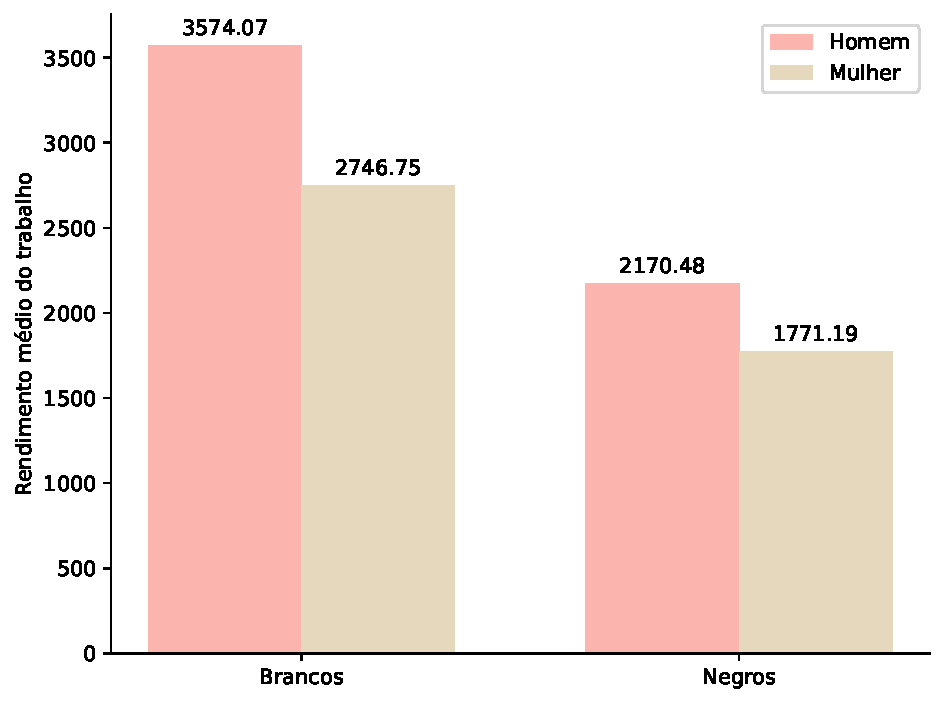
\includegraphics[height=8cm]{/home/dell/Documents/pacto/reports/black_women/figures/wage_2002_group.pdf}
    \label{fig:rendimento_trabalho}
\end{figure}

\par Um outro fato estilizado é que as diferenças salarials nos sub-grupos demográficos analisados possui forte heterogeneidade regional.\footcite{campante2004desigualdade}. Neste sentido, o que a literatura têm mostrado é que as desigualdades salariais são muito mais pronunciadas no Nordeste que no Sudeste. A \ref{fig:rendimento_regiao} ilustra este fato. Fica claro que no Nordestea discrepância salarial entre brancos e negros é muito maior que a diferença observada no Sudeste. Este efeito também aparece quando considera-se apenas as mulheres, já que no Nordeste a mulher negra recebe, em média, 61,7\% do rendimento de um homem branco, enquanto no Sudeste essa razão é de 46,5\%.


\begin{figure}[H]
    \centering
    \caption{Rendimento médio do trabalho - Sudeste e Nordeste - 2022}
        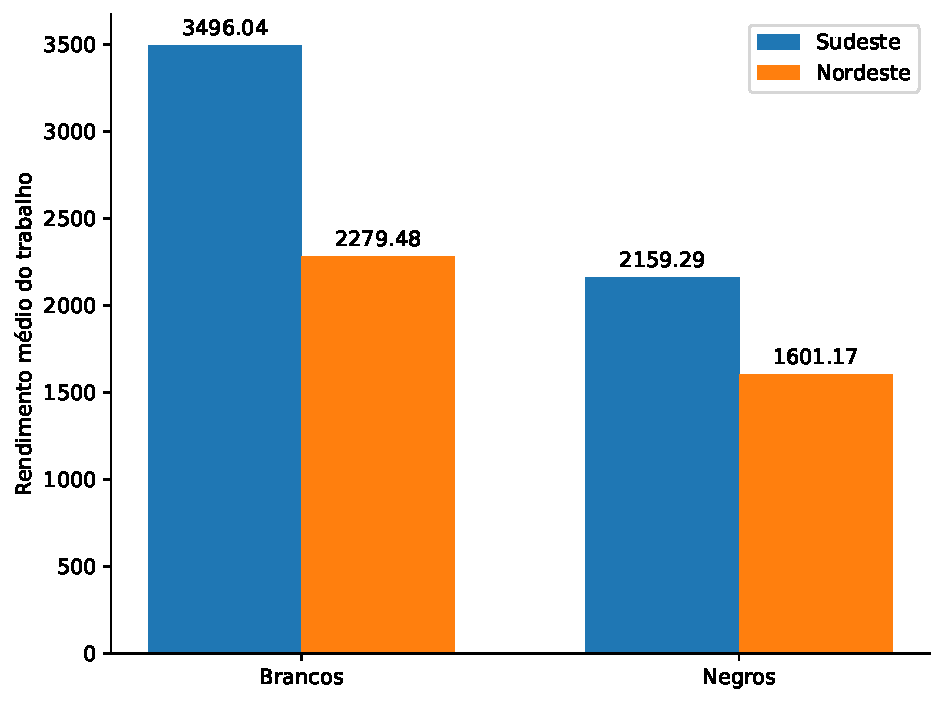
\includegraphics[height=8cm]{/home/dell/Documents/pacto/reports/black_women/figures/wage_2002_region.pdf}
    \label{fig:rendimento_regiao}
\end{figure}

\par Uma fonte adicional de heterogeneidade nos diferenciais salariais entre brancos e negros é o nível de renda. Estudos mostram que quanto maior o nível do extrato de renda, maior é a parcela do diferencial de renda de brancos e negros que não é explicada por variáveis observadas. Esta característica dos diferenciais salariais por cor da pele no mercado de trablho brasileiro é conhecida na literatura como \textit{discriminação elitista}.\footcite[]{soares2000perfil,campante2004desigualdade}

\begin{table}[htb!]
    \centering
    \caption{Distribuição de rendimentos por sexo e cor - Brasil 2022}
    \begin{tabular}{lcccc}
    \hline
    Decil & \multicolumn{2}{c}{Brancos} & \multicolumn{2}{c}{Negros} \\ \cline{2-5} 
          & Homens      & Mulheres      & Homens      & Mulheres     \\ \hline
    10\%  & 1212        & 916           & 800         & 550          \\
    50\%  & 2000        & 1700          & 1500        & 1250         \\
    90\%  & 7500        & 5000          & 4000        & 3000         \\
    99\%  & 25000       & 17500         & 12000       & 9000         \\ \hline
    \end{tabular}
    \label{tab:decis}
    \begin{floatnotes}
      \item[Fonte:] Pesquisa Nacional por Amostra de Domicílios Contínua. 2º trimestre/2022.
      \item[Notas:] Para o cálculo, foram considerados apenas rendimento do trabalho de pessoas ocupadas com idade entre 14 e 65 anos.
  \end{floatnotes}
    \end{table}

% fazer tabela com distribui;'ao por percentil selecionado. Destacar que para maiores percentis, distância é maior
% mostrar que diferen;a no setor p[ublico é menor
% mostrar questão de empregabilidade
% mostrar gap educacional
%


\par Os fatos estilizados apresentados acima são baseados na literatura existente.\footnote{Para os fatos estilizados de 1-4, ver \cite{soares2000perfil}} Embora esses fatos tenham o benefício de apresentar um quadro geral sobre as condições de participação da mulher negra no mercado de trabalho, a mera revisão da literatura existente falha em apresentar um quadro coeso e atualizado da situação da mulher negra no mercado de trabalho. Isso ocorre tanto em função de recortes temporais feitos por pesquisas mais antigas, quanto pelo foco escolhido por cada pesquisador no mercado de trabalho, seja formal ou informal. Com o objetivo de atualizar os dados apresentados pela literatura existente e abarcar tanto o mercado formal quanto o mercado informal de trabalho, esta seção apresenta dados atualizados dos fatos destacados pela literatura existente usando as duas principais bases administrativas do mercado de trabalho brasileiro, RAIS e PNAD.

\par Começa-se, assim, por avaliar o primeiro fato estilizado. As tabelas X e Y apresewntam, respectivamente, a média salarial de homens negros, mulheres brancas, mulheres negras e homens brancos usando dados da PNAD e RAIS. O dado da PNAD é mais atualizado e refere-se ao trimestre X de 2022, enquanto o dado da RAIS refere-se estritamente ao mercado formal de trabalho e cobre o ano de 2020.




\section{Representatividade e educação no mercado formal de trabalho} 

\par Na seção anterior, viu-se que XYZ. Nesta seção, procura-se analisar a evolução da participação da mulher negra no mercado de trabalho entre 2010 e 2020. Como ponto de partida para a disucussão, usa-se o Índice ESG de Equidade Racial (IEER), métrica elaborada pelo Pacto pela Equidade Racial e utilizada por diversas empresas parceiras. Uma discussão completa sobre o IEER e suas propriedades pode ser encontrada no site Pacto.

\par O primeiro resultado apresentado é o IEER atual das mulheres negras no mercado de trabalho forma brasileiro. Antes de apresentar os resultados, porém, é importante destacar uma questão relacionada à interpretação do IEER. O IEER, originalmente, mensura o número de desvios padrões em que o número de negros em determinada ocupação supera o valor esperado de negros dado uma população de referência. Esse valor, contudo, passa por uma transformação algébrica, com o objetivo de comparar o índice entre diferentes ocupações e empresas e fixar seu intervalo em [-1,1]. A transformação algébrica viabiliza a interpretação relativa, ao custo de limitar a possibilidade de interpretação absoluta do índice. Por essa razão, o valor do índice não pode ser interpretado em termos absolutos e, em particular, não tem uma interpretação de \enquote{elasticidade}. Um setor, por exemplo, com IEER=-0,32 não tem 32\% a menos de negros do que seria esperado. Esta é uma interpretação errada.

\par Por outro lado, a magnitude do valor absoluto do índice mostra sim \textit{o grau} de sub ou sobre-representação de negros na unidade produtiva. Assim, por exemplo, um empresa com IEER=-0.8 tem uma desigualdade racial nas suas ocupações \textit{maior} que uma empresa com IEER=-0.6. Para ajudar na interpretação dos valores do IEER, os autores do índice de equidade ocupacional, que serve de base para o IEER, sugeriram a seguinte classificação.\autocite{ransom2001one}

\begin{table}[htb!]
\centering
\caption{Interpretação dos intervalos do Índice ESG de Equidade Racial}
\begin{tabular}{lc}
\hline
Grupo             & Intervalo                 \\ \hline
Não-Mulher Negra Excluídos & $IEER \geq 0, 8 $               \\
Dominância Mulher Negra  & $0,2 < IEER < 0,8$   \\
Equidade          & $-0,2\leq IEER \leq 0,2$  \\
Dominância Não-Mulher Negra & $-0,8 < IEER < -0,2$ \\
Mulher Negra Excluída  & $IEER \leq -0,8$        \\ \hline
\end{tabular}
\end{table}

\par Os valores apresentados na tabela \ref{tab:ieer_2020} mostram, então, que mulheres negras estão sub-representadas no mercado de trabalho formal brasileiro em uma proporção em que é possível falar em \textit{dominância} dos demais grupos demográficos, mas não \textit{exclusão} de mulheres negras. Chega-se a essa interpretação ao se observar o valor do IEER Ponderado, principal indicador na tabela \ref{tab:ieer_2020}. Os demais IEERs mostram a situação de representatividade de mulheres negras em 3 grupos de ocupação, não-liderança, gerência e diretoria. Fica claro que a representação de mulheres negras é maior em ocupações de não-liderança e diminui a medida que se avança no nível hierárquico das ocupações. Os resultados da tabela \ref{tab:ieer_2020} referem-se a trabalhadores formais de todas as empresas brasileiras em 2020. É possível que os resultados observados variem quando se considera heterogeneidades regionais e econômicas das empresas.

\begin{table}[htb!]
    \centering
    \small
    \caption{Índice ESG de Equidade Racial - Mulheres Negras - 2020}
    \begin{tabular}{lc}
    \hline
    \multicolumn{1}{c}{Grupo} & IEER   \\ \hline
    Não-Liderança             & -0.579 \\
    Gerência                  & -0.656 \\
    Diretoria                 & -0.760 \\
    Ponderado                 & -0.665 \\ \hline
    \end{tabular}
    \label{tab:ieer_2020}
    \begin{floatnotes}
    \item [Fonte:] RAIS 2020.
    \item [Nota:] A população de referência utilizada é igual à metade da população de pretos e pardos.
    \end{floatnotes}
    \end{table}

\par Como a situação de representatividade da mulher negra de hoje se compara com a última década? Esta pergunta é respondida pela figura \ref{fig:ieer_evolution} que apresenta a evolução do IEER Ponderado e dos IEERs ocupacionais de 2010 a 2020. Fica evidente que há uma evolução favorável no sentido de aumento da representação de mulheres negras nos últimos 10 anos. O resultado, que aparece no IEER Ponderado, é consequência da evolução favorável dos 3 IEERs ocupacionais, inclusive diretoria. Em que pese o fato da sub-representação de mulheres negras ser ainda muito elevada em 2020, como visto na tabela \ref{tab:ieer_2020}.

\begin{figure}[H]
    \centering
    \caption{Evolução do IEER Ponderado - Mulheres Negras - 2010/2020}
        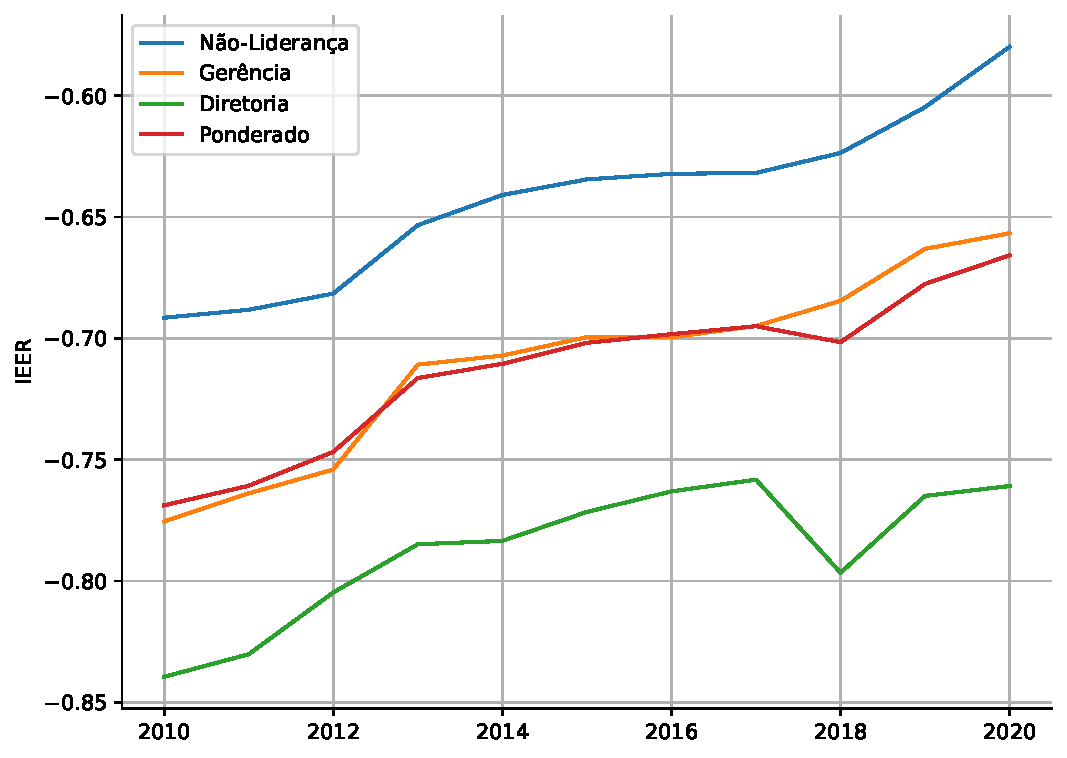
\includegraphics[height=8cm]{/home/dell/Documents/pacto/reports/black_women/figures/ieer_black_women.pdf}
    \label{fig:ieer_evolution}
\end{figure}

\par O IEER é uma medida de representatividade que leva em conta a desigualdade salarial. Isto porque o indicador de desigualdade ocupacional que serve de base para o IEER é ponderado pela massa salarial, dando maior peso a ocupações com maior nível salarial. Dessa forma, seria possível que parte da melhora observada na figura \ref{fig:ieer_evolution} fosse causada pela queda da desigualdade salarial no período. A figura \ref{fig:wage_gap} mostra, porém, que este não é o caso. Na figura, observa-se a evolução da proporção do salário de homens negros, mulheres brancas e mulheres negras em relação ao salário de homens brancos. Fica claro a estagnação dos salários relativos de mulheres negras que, no período, perceberam aproximadamente 55\% do salário recebidos por homens brancos.

\begin{figure}[H]
    \centering
    \caption{Evolução do salário relativo em relação aos homens brancos - 2010/2020}
        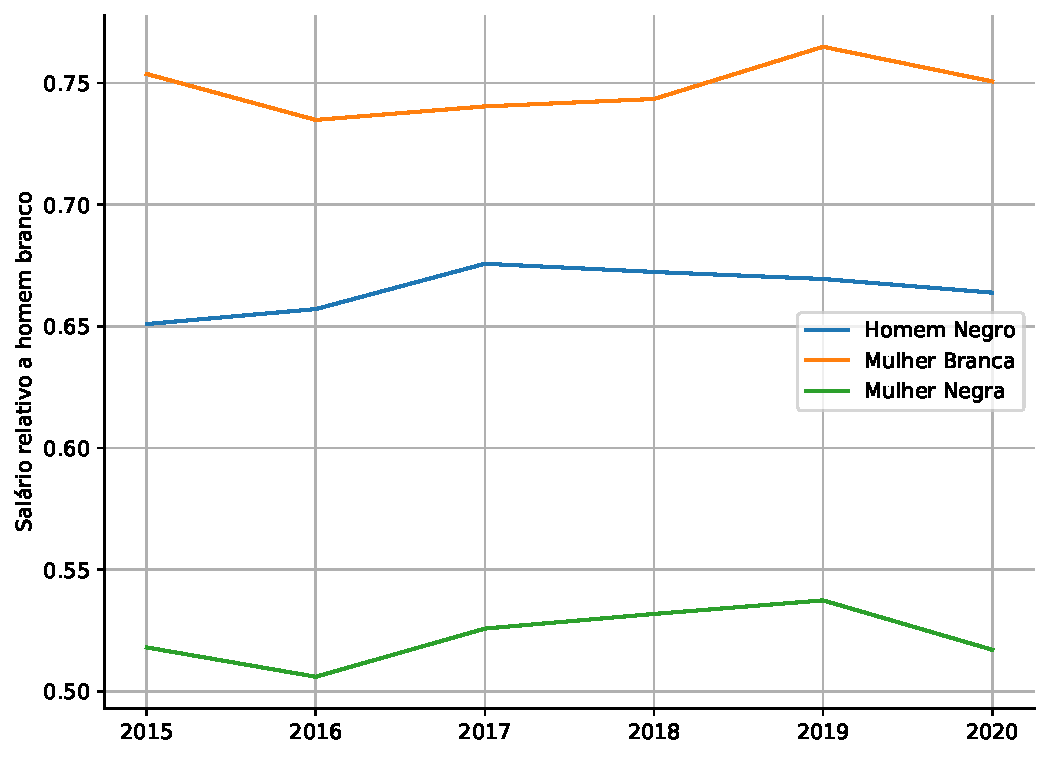
\includegraphics[height=8cm]{/home/dell/Documents/pacto/reports/black_women/figures/wage_gap.pdf}
    \label{fig:wage_gap}
\end{figure}

\par A figura \ref{fig:supply_gap} mostra que, de fato, a provável explicação da melhora do IEER das mulheres negras na última década esteja no aumento do quantitativo de trabalhadores negros no mercado de trabalho formal no período. A figura que, em relação a homens brancos, o número de mulheres negras com carteira assinada avançou cerca de 30 pontos percentuais, saindo de aproximadamente 30\% em 2010 e alcançando pouco mais de 50\% em 2020.


\begin{figure}[H]
    \centering
    \caption{Evolução da participação no mercado de trabalho formal em relação ao homem branco - 2010/2020}
        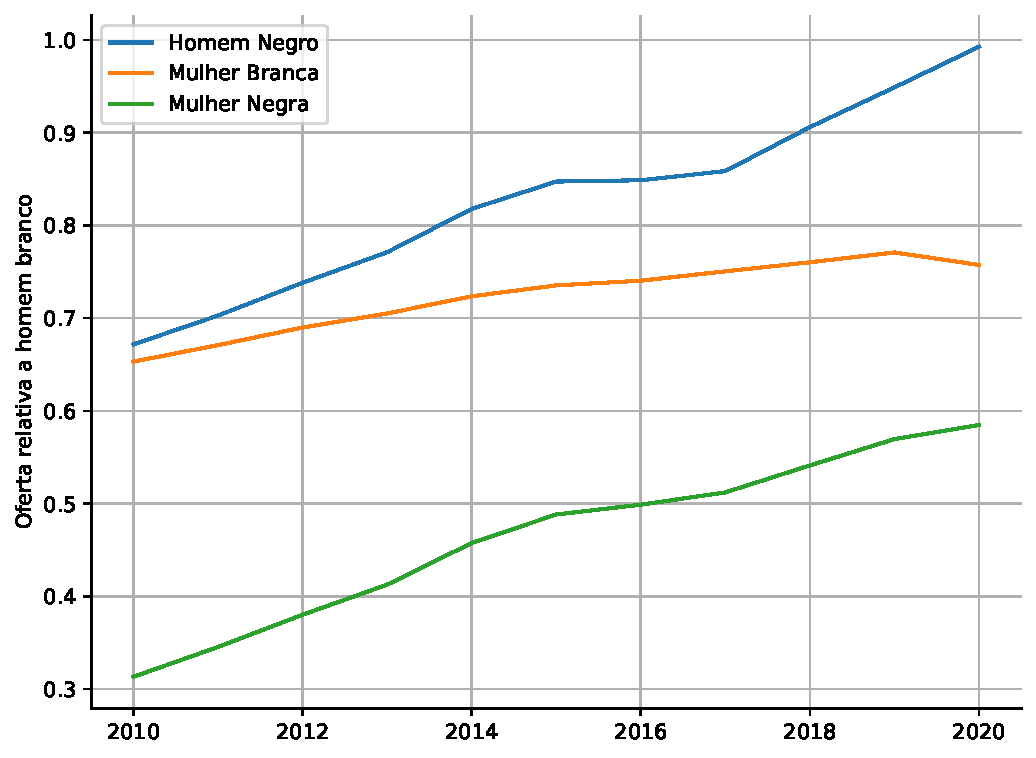
\includegraphics[height=8cm]{/home/dell/Documents/pacto/reports/black_women/figures/supply_gap.pdf}
    \label{fig:supply_gap}
\end{figure}

\begin{table}
\centering
\caption{Composição educacional da oferta de trabalho de mulheres negras - 2010-2020}
\begin{tabular}{lrrr}
\toprule
{} &  Até Fundamental &  Ensino Médio &  Superior+ \\
ano  &                  &               &            \\
\midrule
2010 &            23.9\% &         63.1\% &      13.0\% \\
2011 &            22.4\% &         64.5\% &      13.1\% \\
2012 &            21.3\% &         65.3\% &      13.4\% \\
2013 &            20.2\% &         65.9\% &      14.0\% \\
2014 &            18.5\% &         66.5\% &      15.0\% \\
2015 &            17.7\% &         66.6\% &      15.8\% \\
2016 &            16.3\% &         66.0\% &      17.7\% \\
2017 &            15.0\% &         66.3\% &      18.7\% \\
2018 &            14.0\% &         65.8\% &      20.1\% \\
2019 &            13.2\% &         66.4\% &      20.4\% \\
2020 &            12.4\% &         66.8\% &      20.8\% \\
\bottomrule
\end{tabular}
\end{table}

\begin{table}[htb!]
\centering
\caption{Composição educacional da oferta de trabalho de homens negros - 2010-2020}
\begin{tabular}{lrrr}
\toprule
{} &  Até Fundamental &  Ensino Médio &  Superior+ \\
ano  &                  &               &            \\
\midrule
2010 &            45.8\% &         48.5\% &       5.7\% \\
2011 &            43.3\% &         50.8\% &       5.9\% \\
2012 &            40.9\% &         52.6\% &       6.5\% \\
2013 &            38.6\% &         54.6\% &       6.8\% \\
2014 &            36.1\% &         56.5\% &       7.5\% \\
2015 &            33.9\% &         58.3\% &       7.8\% \\
2016 &            31.5\% &         59.3\% &       9.2\% \\
2017 &            29.3\% &         61.2\% &       9.6\% \\
2018 &            28.0\% &         62.0\% &      10.0\% \\
2019 &            26.8\% &         63.2\% &      10.0\% \\
2020 &            25.7\% &         64.2\% &      10.1\% \\
\bottomrule
\end{tabular}
\end{table}


\begin{figure}[H]
    \centering
    \caption{EComposição educacional força de trabalho- Mulheres Negras - 2010/2020}
        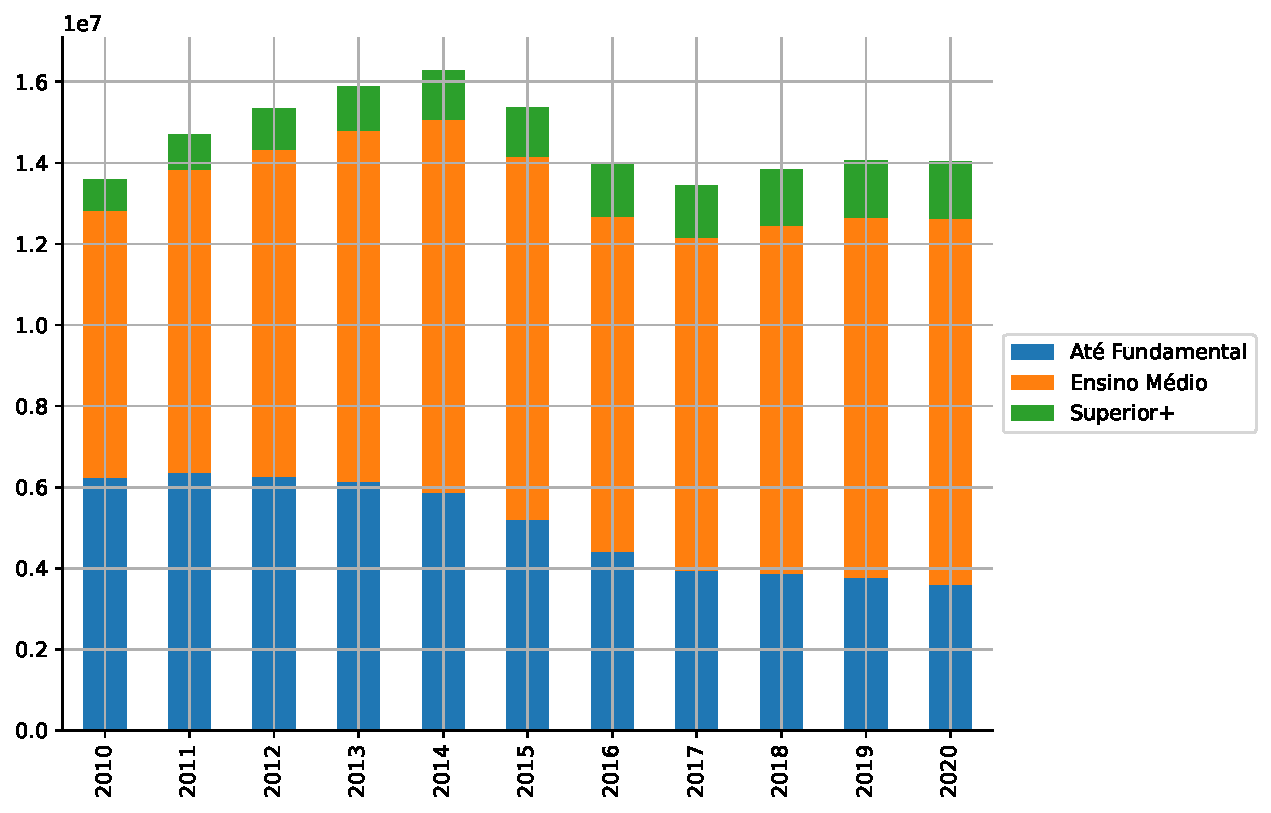
\includegraphics[height=8cm]{/home/dell/Documents/pacto/reports/black_women/figures/education_main_groups.pdf}
    % \label{fig:ieer_evolution}
\end{figure}

\section{Conclusão}

\clearpage

\printbibliography[title={Bibliografia}, nottype=misc]

\end{document}